\chapter{Source detection in radio astronomy}\label{C:intro}
The sheer volume of data to be produced by next generation radio telescopes makes automated methods for the detection of astronomical objects (``sources") essential. Current methods require time-intensive parameter tuning and do not find all sources, particularly scientifically interesting low surface-brightness objects.

This thesis explores Bayesian methods that use Dirichlet or multinomial models for pixel intensity distributions in source detection in discretised radio astronomy images.

The methods developed in this thesis exploit the consistency of image background, while minimising the problems inherent in modelling the diversity of astronomical objects. The posterior probability that a given region is source or background is inferred, avoiding the difficulties in approaches based on comparing ``typical" exemplars of source and background.

\section{Source detection in radio astronomy}
Existing automated approaches to detecting scientifically important astronomical objects require time-intensive manual parameter tuning, and manual post-processing by an astronomer. The sheer volume of data to be produced by the next generation of radio telescopes --- exabytes of data on hundreds of millions of objects --- will make efficient and timely detection of astronomical objects by such manually intensive processing at best impracticable and at worst impossible. Fully automated approaches that do not require manual tuning and post-processing are therefore essential to finding objects of interest in astronomical images \cite{norris2011emu}.

Further, current algorithms for automatic source detection are not fully adequate to find all objects of interest. Spatially extended sources, particularly those that are faint, are poorly handled by existing automated approaches, as are sources in the presence of artefacts, and sources in images in which the signal-to-noise ratio varies across the image \cite{hollitt2012feature, norris2011emu, norris2012radio}.

\subsection{Characteristics of radio astronomy images}

Radio astronomy images can be thought of as primarily background with an unknown number of spatially extended sources. Identifying the sources requires distinguishing them from background, a task made difficult by the diversity of pixel intensities within and between sources. In general, source pixels are brighter than background pixels, though there is considerable overlap between background and source intensity ranges. 

The intensity of background pixels in radio telescope images is non-uniform, but follows a Gaussian distribution in local areas. The variability of background however is lower than that of sources and in that sense it is easier to identify.

The noise in radio astronomy images varies over an image. Images typically display more noise around their edges (for example, see Figure \ref{fig:background-var} in Chapter \ref{C:1D}).

Sources in radio astronomy images can be divided into the following classes:
\begin{itemize}
\item Point sources (Figure \ref{fig:pointsource}), which are unresolved sources in an image; at or below the resolution
element of a telescope. Point sources are abundant in radio astronomy images. They are relatively bright and not spatially extended, and are well-found by existing algorithms\footnote{Hancock \textit{et. al.} \cite{hancock2012compact} report that $\sim 99\%$ of point sources are found by widely used source detection packages (that is, a $\sim 1\%$ false negative rate); similarly $\sim 99\%$ of reported point sources are actual point sources (a $\sim 1\%$ false positive rate).}.
\item Galaxy clusters and associated structures, which are of interest to astronomers. These include:
	\begin{itemize}
	\item Radio galaxies consist of a small, circular, central source from which two, roughly symmetrical, elliptical lobes emanate 180 degrees from each other. The central source is typically brighter than the lobes. Radio galaxies such as the linear source Centaurus A (Figure \ref{fig:centa}) may be bright and extended, or they may be diffuse, extended, low surface brightness sources. One or more of the lobes or central source may be absent or may be distorted. A galaxy's symmetry may be distorted, and lobes may be warped and may differ in size, shape, and brightness. One lobe may appear brighter than the other. Unrelated objects (for example, point sources) may appear on or near the galaxy. Tailed radio galaxies are a sub-class of radio galaxies (Figure [REF]). 
	\item Radio relics (found on the periphery of clusters) appear as dim, diffuse, extended single or double arcs (Figure \ref{fig:radio-relic}).
        \item Radio halos (found around the centres of galaxy clusters) are diffuse, circular structures.
	\end{itemize}
\item Supernova remnants (SNRs; Figure [REF]) are also of interest to astronomers. SNRs generally appear as hollow circular rings, although regions of the rings are often occluded, and symmetry may be distorted. Old and near SNRs appear faint, diffuse and large in images. Young and distant SNRs may be miss-classified as point sources.
\end{itemize}

Artefacts in images appear as bright circles, rings and radial lines. Artefacts will be less prevalent in next generation radio telescope images, due to the increased number of elements in next generation arrays \cite{norris2011emu}. 

A number of characteristics of astronomical objects of interest to astronomers make the object-detection task non-trivial. These include distorted symmetry and other variations in the appearance of sources, occlusions, and low surface-brightness, particularly in diffuse objects with intensities close to noise.

\begin{figure}
\centering
\makebox[\textwidth][c]{\includegraphics[width=1.0\textwidth]{IMAGES/pointsource.png}}
\caption[Point source]{\textbf{A point source}. The red contours show the $1.4$ GHz radio data and the blue show the $2.4$ GHz data overlaid on the optical image from the Digitized Sky Survey. The resolution of these radio data are $8.8 \times 4.6$ arcseconds at position angle of $2.4$ degrees and $5.0 \times 2.6$ arcseconds at $2.5$ degrees at $1.4$ and $2.4$ GHz, respectively. Despite that the optical host galaxy is clearly seen the radio data are unresolved at both frequencies and so this is a point source in a radio image \cite{johnston2008radio}.}
\label{fig:pointsource}
\end{figure}

\begin{figure}
\centering
\makebox[\textwidth][c]{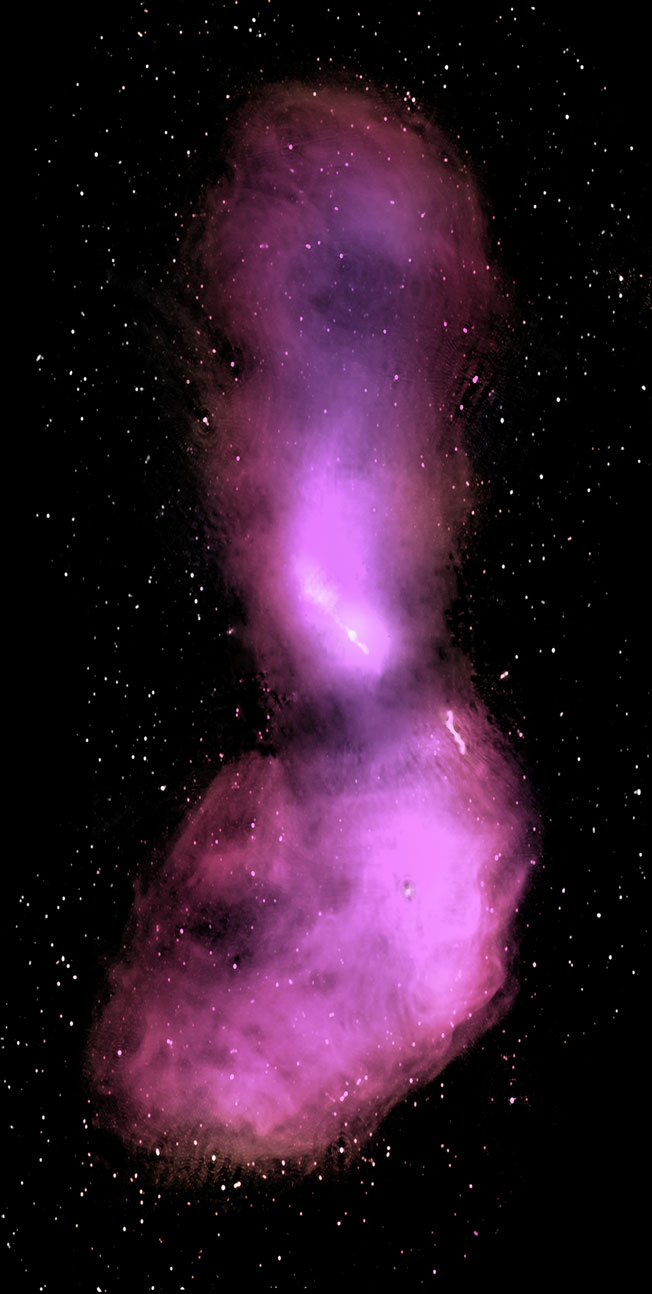
\includegraphics[width=0.7\textwidth]{IMAGES/casa2_lg.jpg}}
\caption[Radio galaxy]{\textbf{A radio galaxy}. Centaurus A is the nearest powerful radio galaxy of the Fanaroff-Reilly class 1 radio galaxies, which typically have jets at 180 degrees \cite{feain2011radio}. }
\label{fig:centa}
\end{figure}


%[Tailed radio galaxy] The tailed radio galaxy PKS J0334-3900

\begin{figure}
\centering
\makebox[\textwidth][c]{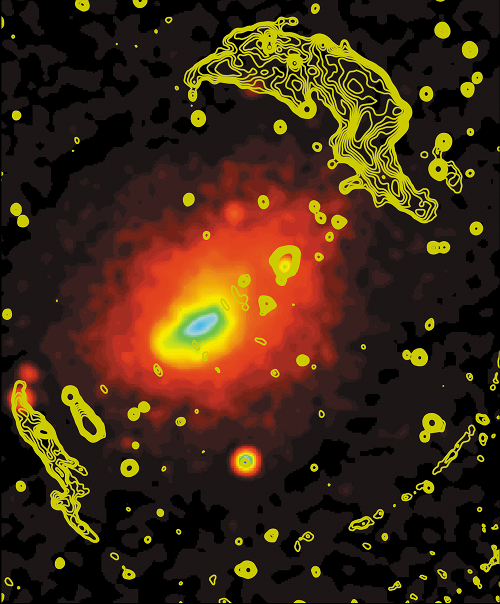
\includegraphics[width=1.0\textwidth]{IMAGES/radio-relics.jpg}}
\caption[Radio relic]{\textbf{A radio relic}, shown by yellow contours \cite{johnston2003detection}.}
\label{fig:radio-relic}
\end{figure}

%SNR figure \cite{zanardo2013high}


\subsubsection{Image format}

Radio telescope images are typically stored in FITS (Flexible Image Transportation System) format. For the astronomical images used in this thesis, image data is stored in two dimensional arrays of pixel intensities with implicit Cartesian coordinates. Pixel intensity values are continuous, and range from small positive to small negative values in any given image. Image meta-data including information about the equatorial coordinates of the image is also stored with this format \cite{wells1981fits}. 

\subsection{Existing approaches to source detection}

An ideal source-finding algorithm should locate regions in an image that differ from the background and are unlikely to have arisen by statistical variation in noise. False positives are more acceptable than than false negatives (as astronomers can do post-processing to confirm and characterise sources), however, a large number of false positives would make output difficult to interpret at best and unusable at worst.

In a 2012 review, Masias \emph{et. al.} \cite{masias2012review} characterised current approaches to automated and semi-automated source detection in astronomy as a two-step process: an image transformation step followed by a detection step. 

Masias \emph{et. al.} divided approaches in the transformation step into basic transformation methods, Bayesian approaches, matched filtering, and multi-scale approaches. Basic transformation methods predominate, and include median filtering, local thresholding using information such as pixel intensity mean and standard deviation, Gaussian image convolution, dilation and erosion, and template matching.

Bayesian approaches transform pixel intensity data to a probability map indicating regions where sources are likely to be located (for example: \cite{feroz2008multimodal}; also see Section \ref{sec:Bayesian-src-det} below). Matched filtering involves convolving an image using an expected source profile as a filter (for example: \cite{torrent2010detecting}), while multi-scale approaches work by applying a transform to decompose images into different frequencies (for example: \cite{peracaula2011segmentation}). 

In the detection step Masias \emph{et. al.} categorised the majority of methods into thresholding (local or adaptive) and local peak search (region growing from peaks in, for example, pixel intensities). The authors also list a small number of ``other" techniques (neural networks, watershed transform, contrast radial function, and connected component trees).

The majority of automated source detection algorithms can therefore be described as flood-filling or region-growing driven by (possibly transformed) pixel intensities \cite{masias2012review}.

Such intensity based thresholding algorithms often require a parameter to be set (either manually or automatically as part of the algorithm) that restricts the sources to be found as those that are at least as bright as some threshold: typically $3 \sigma$ or $5 \sigma$ above root mean square (rms) noise. However, as noted earlier in this chapter, some of the most scientifically important objects in astronomy are dim, low surface brightness sources, with intensities in the range of background noise \cite{norris2011emu}. Restricting the search for sources that contain pixels above a particular threshold restricts the set of sources that may be found. This is due to the nature of thresholding algorithms: if the search is not restricted in this way, far too many background regions will be identified as ``sources", and the output will be unusable.

Threshold-based algorithms are often reported to have very high rates of true detections with very low rates of false detections and missed sources. However, these rates must be taken with caution, as they are often restricted to the sub-set of sources in an image above a particular brightness. For example, Hancock \textit{et. al.} \cite{hancock2012compact} report perfect detection rates with no false detections or missed sources --- in the case of simulated point sources $10 \sigma$ above rms noise. 

The source detection algorithms developed in this thesis are evaluated against two source detection software packages commonly used in radio astronomy: Duchamp \cite{whiting2012duchamp} and BLOBCAT \cite{hales2012blobcat}; both of which perform pixel-intensity based thresholding in the transformation step and flood-filling in the detection step.

\subsection{Bayesian source detection methods}\label{sec:Bayesian-src-det}

Beside the many thresholding and flood-filling / region-growing algorithms, there are a small number of Bayesian source detection algorithms \cite{masias2012review}.

Most of these Bayesian source detection algorithms use Markov-chain Monte Carlo sampling (MCMC) to estimate the relative probability that each pixel (or pixel grouping) in an image is a background pixel or a source pixel \cite{feroz2008multimodal, masias2012review}. 

Savage and Oliver \cite{savage2007bayesian} used MCMC for source detection in infrared astronomical images. Each pixel was labelled with the relative probability of being a background pixel or a source pixel, with a flat and uniform background model, and a source model consisting of background plus a circularly symmetric Gaussian point source of known size. This labelling yields a probability map which can be used to find local maxima (subject to some threshold) corresponding to locations of point sources. Once the location of putative sources is found by this method, the nature of the source is identified: MCMC sampling is used to find the best-fit model of uniform background, point source, or extended source models (where point sources are circularly symmetric and of known size, and extended sources are circularly symmetric with variable size).  

Similarly, Hobson and McLachlan \cite{hobson2003bayesian} performed Bayesian model selection using MCMC to explore the parameters of background and source models, with a source model of circularly symmetric Gaussian-shaped objects and a background model of Gaussian noise. They present two versions of the algorithm: one in which all sources are found simultaneously, and one in which sources are found iteratively. A significant speed up to this technique is presented in Carvalho \textit{et. al.} \cite {carvalho2009fast}, in which multiple local maximisation of the posterior distribution replaces sampling, and a Gaussian approximation to the posterior is used for the evaluation of Bayesian evidence in model selection.

Guglielmetti \textit{et. al.} \cite{guglielmetti2009background} developed a Bayesian source detection method for X-ray data. They used a two component mixture model where an astronomical image is assumed to consist of a smooth background with additive source signal; therefore the two models are $1.$ background plus noise and $2.$ background plus source plus noise.

Feroz and Hobson \cite{feroz2008multimodal} developed one of the few non-MCMC based Bayesian source detection algorithms. They used the Bayesian model selection algorithm nested sampling \cite{skilling2004nested}, which they argue outperforms MCMC based methods, and is computationally less expensive. Similarly to other Bayesian source detection methods, circularly symmetric Gaussian-shaped sources are assumed.

The Bayesian source detection methods developed in this thesis have some similarities with the existing algorithms in astronomy. For example, in Chapter \ref{C:LDA}, in latent Dirichlet allocation (LDA), Gibbs sampling is performed on individual pixels which are probabilistically assigned background or source labels, with flood-filling performed on the transformed image to identify islands of source pixels. In Chapters \ref{C:1D} and \ref{C:2D}, a Bayesian score (``DM-Score") is derived to iteratively find Gaussian elliptical shaped regions that conform to a source model (or differ from a background model).

In contrast to the existing Bayesian source detection methods however, source and background are modelled as distributions over ranges of pixel intensities. As with the existing Bayesian algorithms, the DM-Score assumes a parametrised form for astronomical sources and estimates these parameters from a posterior distribution, however sources are not assumed to be circularly symmetric or of a particular size. Under LDA, no particular size or shape of sources is assumed.

It is worth noting that in several cases, these Bayesian source detection methods are tested on simulated data in which the sources are generated with the same parameters as the model of source used in the detection methods. For example \cite{feroz2008multimodal,hobson2003bayesian,savage2007bayesian} generate circularly symmetric Gaussian sources of a particular size, and use a circularly symmetric Gaussian of that size as a source model. Using the same parameters for simulated source and the method's source model is likely to artificially inflate the success of the model, and is unjustified in the case of radio astronomy data, where sources can take a great variety of shapes and sizes.

\section{Outline of the thesis}

Within the framework provided by Masias \emph{et. al.} \cite{masias2012review}, the source detection algorithms in this thesis can be characterised as follows:
\begin{itemize}
\item \textbf{Image transformation step}: the continuous valued pixel intensities in astronomical images are converted to discrete values by histogram binning or discretisation. This process is described in \textbf{Chapter \ref{C:BIN}}.
\item \textbf{Detection step}: two approaches are taken:
    \begin{itemize}
    \item Background and source models are inferred using the topic modelling technique latent Dirichlet allocation, these models are used to classify pixels according to which model they were most likely generated by. Flood-filling is then performed to find contiguous regions of ``likely to be source" pixels. The use of LDA for source detection is described in \textbf{Chapter \ref{C:LDA}}. Results of this technique as compared to results obtained by a standard source-detection package are presented.
    \item A Dirichlet-multinomial ``score" (DM-Score) is derived, and, given a background model and a loosely specified source model, gradient ascent is performed to find peaks in the score indicating regions that are unlikely to be background. The derivation of the DM-Score is outlined in \textbf{Chapter \ref{C:1D}}. Results of the DM-Score on real and simulated data are presented in  \textbf{Chapter \ref{C:2D}}.
\end{itemize} 
\end{itemize} 

A combined LDA DM-score technique is described and evaluated in \textbf{Chapter \ref{C:2D-LDA}}. The work in the thesis and its limitations are summarised and possible future work suggested in \textbf{Chapter \ref{C:con}}.

\section{Original contributions}

The contributions of this thesis are as follows:
\begin{itemize}
\item A novel method for incorporating uncertainty about where bin borders should be located in discretised data is introduced in \textbf{Chapter \ref{C:BIN}}.
\item The first use of the topic modelling technique latent Dirichlet allocation (developed to extract latent topics from collections of documents) in source detection in astronomical images is described in \textbf{Chapter \ref{C:LDA}}. This application of LDA to source detection differs from that taken in previous approaches to the segmentation of non-astronomical images in that it relies only on pixel intensity and location, whereas previous approaches employ techniques to extract image interest points and pre-segment images before applying LDA.
\item A new Dirichlet-multinomial score, indicating how well a region conforms to a model of background versus a model of foreground is derived in \textbf{Chapter \ref{C:1D}}.
\item LDA output is utilised in the DM-Score in \textbf{Chapter \ref{C:2D-LDA}}.
\end{itemize}
